\documentclass[]{article}

%opening
\title{4M24 CW - High-Dimensional MCMC}
\author{Candidate: 5562E}

%packages
\usepackage[margin=0.5in]{geometry}
\usepackage[export]{adjustbox}
\usepackage{algorithm}% http://ctan.org/pkg/algorithm
\usepackage{algpseudocode}% http://ctan.org/pkg/algorithmicx
\usepackage{mathtools}
\usepackage{graphicx}
\usepackage{amsmath}
\usepackage{amssymb}
\usepackage{hyperref}
\usepackage{caption}
\usepackage{subcaption}
\usepackage{parskip}
\usepackage{listings}
\usepackage{pdfpages}
\usepackage{bbm}
\usepackage{multirow}

%package setup
\graphicspath{{./img/}}
\DeclareMathOperator*{\argmax}{arg\,max}
\DeclareMathOperator*{\argmin}{arg\,min}

%custom commands
\newcommand{\figwidth}{0.4\linewidth}
\newcommand{\Fcal}{\mathcal{F}}
\newcommand{\idft}{\mathcal{F}^{-1}}
\newcommand{\Xcal}{\mathcal{X}}
\newcommand{\Ncal}{\mathcal{N}}
\newcommand{\Acal}{\mathcal{A}}
\newcommand{\Bcal}{\mathcal{B}}
\newcommand{\cmplx}{\mathbb{C}}
\newcommand{\Lcal}{\mathcal{L}}
\newcommand{\lik}{\lambda}
\newcommand{\loglik}{\Lambda}
\newcommand{\Mcal}{\mathcal{M}}
\newcommand{\indep}{\perp \!\!\! \perp}
\newcommand{\iid}{\stackrel{iid}{\sim}}
\newcommand{\betaml}{\hat{\beta}^{ML}}
\newcommand{\Expect}{\mathbb{E}}
\newcommand{\cbold}{\boldsymbol{c}}
\newcommand{\tbold}{\boldsymbol{t}}
\newcommand{\xbold}{\boldsymbol{x}}
\newcommand{\ubold}{\boldsymbol{u}}
\newcommand{\vbold}{\boldsymbol{v}}
\newcommand{\wbold}{\boldsymbol{w}}
\newcommand{\zbold}{\boldsymbol{z}}
\newcommand{\epsbold}{\boldsymbol{\epsilon}}
\newcommand{\thetabold}{\boldsymbol{\theta}}
\newcommand{\zetabold}{\boldsymbol{\zeta^*}}
\newcommand{\omegabold}{\boldsymbol{\omega}}
\newcommand{\Rho}{\mathcal{P}}


%section numbering
\renewcommand{\thesubsection}{\alph{subsection}}

\begin{document}


\includepdf[pages={1}]{4M24-Coversheet.pdf}

\setcounter{page}{1}
\maketitle

\begin{abstract}
	This report outlines the result of the 4M24 coursework on high-dimensional Markov Chain Monte Carlo (MCMC). We begin with the classical problem of generating a field from a Gaussian Process. From this field, we subsample and add noise to obtain data which we can use to infer the original field. This inference is performed through a Markov chain which can draw samples from the posterior distribution on the original field given the observed data.
	
	Two algorithms are compared: Gaussian Random Walk - Metropolis Hastings (GRW-MH) and preconditioned Crank-Nicholson (pCN). Both algorithms produce comparably accurate predictions but pCN is preferred for its higher acceptance rate and faster execution.
	
	More information is removed, by transforming the available data to only encode the sign (a probit transform). We apply pCN to infer the original binary field with great success. Furthermore, we are able to infer the original choice of length-scale used to generate the data by minimising the resulting prediction error.
	
	Lastly, we apply these tools to a real-world inference problem: modelling bike theft in the London Borough of Lewisham. pCN is once again used with some modifications to infer the underlying field from subsamples of its realisations. We find good agreement between model and observed data. However, the model's predictive power may be more useful if its length-scale is chosen from sound analysis of the problem a priori. Indeed, choosing the length-scale to minimise the prediction error runs the risk of overfitting to this particular dataset. Nevertheless, a full Bayesian treatment can be applied to augment the prior information with the likelihood information from the realised dataset. 
\end{abstract}

\section{Simulation}
\subsection{Sampling from a Gaussian Process}

We begin with a Gaussian Process (GP) defined on a 2D domain $\xbold \in [0, 1]^2$. The realisations from this process are denoted $\ubold \sim \Ncal(0, C)$ where $C_{ij} = k(\xbold_i, \xbold_j)$ and k is the Squared Exponential (SE) covariance function with length parameter $l$:
%
\begin{equation}
	k(\xbold, \xbold ') = \exp \left( \frac{-||\xbold - \xbold '||^2}{2l^2}\right)
	\label{eqn:k-defn}
\end{equation}

If we specify the latent variables $\{\xbold_i\}_{i=1}^N$, then we can compute $C$ and hence fully specify the prior on $u$. We choose to place $\{x_i\}_{i=1}^N$ on a $D \times D$ grid with equal spacing, starting at $(0,0)$ and ending at $(1,1)$. Obviously, we require $N = D^2$.

We can now plot the $u$-surface atop this grid by ensuring that for each $i \in \{1 \dots N\}$, $u_i$ denotes the Z-position and $\xbold_i$ the X-Y-position. We can then investigate the effect of varying the length-scale parameter $l$. Three settings of $l$ and the associated plots are given in figure \ref{fig:l-effect} for $D=16$.
%
\begin{figure}[!h]
	\centering
	\begin{subfigure}{0.32\linewidth}
		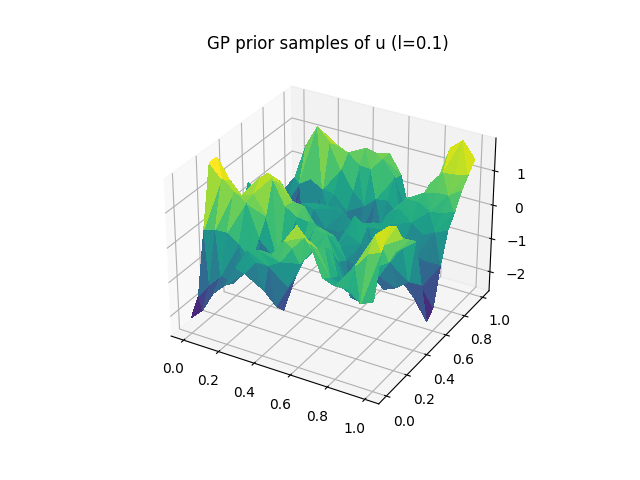
\includegraphics[width=\linewidth]{u-small.png}
		\caption{Small $l=0.1$}
	\end{subfigure}
	\begin{subfigure}{0.32\linewidth}
		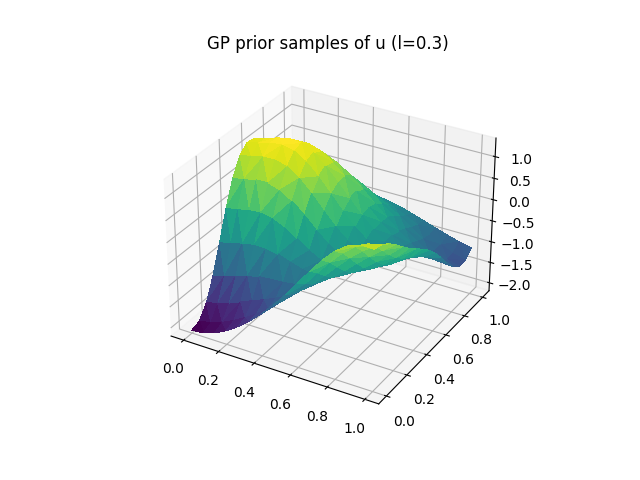
\includegraphics[width=\linewidth]{u-med.png}
		\caption{Medium $l=0.3$}
	\end{subfigure}
	\begin{subfigure}{0.32\linewidth}
		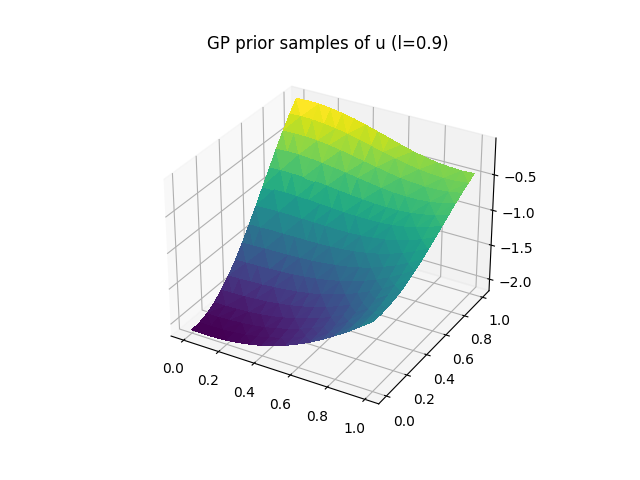
\includegraphics[width=\linewidth]{u-big.png}
		\caption{Large $l=0.9$}
	\end{subfigure}
	\caption{Samples from GP prior for varying length scales ($D=16$)}
	\label{fig:l-effect}
\end{figure}

We now proceed to make $M$ random draws (denoted by the $M \times 1$ vector $\vbold$) from these samples $\ubold$ with additive Gaussian noise $\epsbold \sim \Ncal(0, I)$. The subsampling factor $f$ is defined as $f \coloneqq N / M$. The draws can be computed as follows:
%
\begin{equation}
	\vbold = G \ubold + \epsbold
	\label{eqn:v-defn}
\end{equation}

Where $G$ is an $M \times N$ matrix with a single one in each row in a random location (without repetition) and rest zeros. In what follows, a tilde will denote a subsampled vector such that $\tilde{\ubold} \coloneqq G\ubold$. The result is that the observations $\vbold$ are a jumbled subsample of $\ubold$ with additive noise $\epsbold$. We can plot the data overlaid on the original prior samples by simply matching each entry of $\vbold$ back to the coordinate it was selected from. The result is plotted on figure \ref{fig:v-on-u}.
%
\begin{figure}[!h]
	\centering
	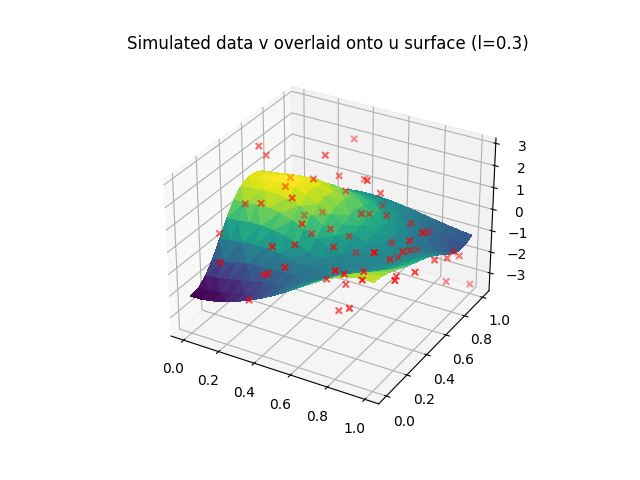
\includegraphics[width=\figwidth]{v-overlay.png}
	\caption{$\vbold$ (red crosses) overlaid on $\ubold$-surface ($f=4, D=16, l=0.3$)}
	\label{fig:v-on-u}
\end{figure}

We observe $M=N/f=16^2/4=64$ samples contained in the $\vbold$ vector. These are equally likely to appear above or below the $\ubold$-surface as the noise has zero mean. The noise variance for each data-point is of similar magnitude to the variation in the surface ($\sigma^2 = 1$) so some crosses appear relatively far away from the surface. Moreover, as the subsampling is random, the $\vbold$-points appear at randomly chosen (but distinct) locations X-Y plane.

\subsection{Log probabilities and MCMC}

We assume that we have realised a set of observations $\vbold$ and it is now our job to determine probability distributions for $\ubold$ based on this information. As a matter of notation, we define the prior function $\pi(\cdot) \coloneqq p(\ubold=\cdot)$ and likelihood function $\lik(\cdot) \coloneqq \ln p (\vbold | \ubold = \cdot)$. Likewise, we define the posterior $\rho(\cdot) \coloneqq p(\ubold=\cdot | \vbold)$.

The log prior can be calculated simply, through manipulation of the Gaussian pdf:
%
\begin{align}
	\ln \pi (\wbold) &= \ln \Ncal(\wbold; 0, C) \ln \frac{1}{(2\pi)^{N/2} |C|^{1/2}} \exp \left( - \frac{1}{2} \wbold^T C^{-1} \wbold \right) \nonumber \\
	&= - \left( \frac{N}{2} \ln 2\pi + \frac{1}{2} \ln |C| + \frac{1}{2} \wbold^T C^{-1} \wbold \right)
	\label{eqn:log-prior}
\end{align}

Likewise, $\vbold | \ubold$ is also a Gaussian such that $\vbold |\ubold \sim \Ncal(G\ubold, I)$ (see equation \ref{eqn:v-defn}). By comparison with the form of equation \ref{eqn:log-prior}, we can jump straight to the log-likelihood, noting that $\ln |I| = 0$:
%
\begin{equation}
	\ln \lik(\wbold) = - \left( \frac{M}{2} \ln 2 \pi + \frac{1}{2} \left(\vbold - G\wbold \right)^T \left(\vbold - G\wbold\right)\right)
	\label{eqn:log-likelihood}
\end{equation}

From these it is trivial to determine the log-posterior from Bayes' rule:
%
\begin{align}
	\rho(\wbold) &\propto \pi(\wbold) \cdot \lik(\wbold) \nonumber \\
	\therefore \ln \rho(\wbold) &= \ln \pi(\wbold) + \ln \lik(\wbold) + \textrm{const}
\end{align}

It is important to note that, $\wbold$ is simply a dummy variable. We can simplify this notation further by defining $\Rho \coloneqq \ln \rho + \textrm{const}$, $\Pi \coloneqq \ln \pi$ and $\loglik \coloneqq \ln \lik$. The constant can be chosen to give us:
%
\begin{equation}
	\Rho(\omegabold) = \Pi(\omegabold) + \loglik(\omegabold)
	\label{eqn:log-posterior}
\end{equation}

\subsubsection{Gaussian Random Walk - Metropolis Hastings (GRW-MH)}

Armed with the log-posterior (equation \ref{eqn:log-posterior}), observations $\vbold$ and observation matrix $G$, we can now apply the Gaussian Random Walk Metropolis-Hastings algorithm to draw samples of $\ubold$ from the posterior. We start with an initial estimate drawn from the prior $\ubold^{(0)} \sim p(\ubold) = \Ncal(\ubold; 0, C)$. For simplicity we use the symbol $\zetabold$ to denote a fresh sample drawn from the prior $\pi \sim \Ncal(0, C)$. It is computed by applying a Cholesky decomposition to the covariance matrix $C$ and multiplying a standard Gaussian vector $\zbold \sim \Ncal(0, I)$. As such:
%
\begin{equation}
	\zetabold = C^{1/2} \zbold
	\label{eqn:zeta}
\end{equation}

To emphasise, every time $\zetabold$ appears in an equation we draw a fresh sample according to equation \ref{eqn:zeta}. We then pick a symmetric proposal distribution to sequentially generate samples. Given a sample $\ubold^{t}$ we generate a proposal $\wbold^{(t)}$ as follows:
%
\begin{equation}
	\wbold^{(t)} \coloneqq \ubold^{(t)} + \beta \zetabold
\end{equation}

Where $\beta$ is a hyperparameter that controls the step-size of each iteration. As our proposal distribution is symmetric, the acceptance probability $\alpha^{(t)} \coloneqq \alpha(\ubold^{(t)}, \wbold^{(t)})$ simplifies to the ratio of posteriors (with an upper bound of 1):
%
\begin{equation}
	\alpha(\ubold, \wbold) \coloneqq \min \left( \frac{\rho(\wbold)}{\rho(\ubold)}, 1 \right)
\end{equation}

It may be more natural to deal in log of this value:
%
\begin{equation}
	\ln \alpha^{(t)} = \min \left(\Rho(\wbold^{(t)}) - \Rho(\ubold^{(t)}), 0\right)
\end{equation}

Note that the constant term in the $\Rho$ definition cancels. Naturally, we can sample a uniform random variable $U \sim \mathcal{U}(0, 1)$ and compare to $\alpha^{(t)}$:
%
\begin{align}
	p(U < \alpha) &= \alpha \nonumber \\
	\therefore p(\ln U < \ln \alpha) &= \alpha
\end{align}

The algorithm for GRW-MH is given in algorithm \ref{alg:grw-mh}.
%
\begin{algorithm}
	\caption{Gaussian Random Walk - Metropolis Hastings}
	\label{alg:grw-mh}
\begin{algorithmic}
	\State $\ubold^{(0)} \gets \zetabold$
	\For{$t \in \{0, 1 \cdots T-1\}$}
	\State $\wbold^{(t)} \gets \ubold^{(t)} + \beta \zetabold$ \Comment{Generate proposal}
	\State $\ln \alpha^{(t)} \gets \min \left(\Rho(\wbold^{(t)}) - \Rho(\ubold^{(t)}), 0\right)$
	\State $U^{(t)} \gets \sim \mathcal{U}(0,1)$ \\
	\If {$\ln U^{(t)} \leq \ln \alpha^{(t)}$}
		\State $\ubold^{(t+1)} \gets \wbold^{(t)}$ \Comment{Proposal accepted}
	\Else
		\State $\ubold^{(t+1)} \gets \ubold^{(t)}$ \Comment{Proposal rejected}
	\EndIf
	\EndFor
\end{algorithmic}
\end{algorithm}

As our algorithm depends only on the difference of the posteriors, there is no need to compute the constant term. This massively speeds up computation.

\subsubsection{Preconditioned Crank-Nicholson (pCN)}

Preconditioned Crank-Nicholson is rather similar, except we choose a subtly different proposal distribution:
%
\begin{equation}
	\omegabold^{(t)} \coloneqq \sqrt{1 - \beta^2} \ubold^{(t)} + \beta \zetabold
\end{equation}

This changes the form of our acceptance probability subtly by exchanging the log-posterior $\Rho$ for the log-likelihood $\loglik$. The rest of the algorithm is broadly unchanged (see algorithm \ref{alg:pCN}).
%
\begin{algorithm}
	\caption{preconditioned Crank-Nicholson}
	\label{alg:pCN}
	\begin{algorithmic}
		\State $\ubold^{(0)} \gets \zetabold$
		\For{$t \in \{0, 1 \cdots T-1\}$}
		\State $\wbold^{(t)} \gets \sqrt{1 - \beta^2} \ubold^{(t)} + \beta \zetabold$ \Comment{Generate proposal}
		\State $\ln \alpha^{(t)} \gets \min \left(\loglik(\wbold^{(t)}) - \loglik(\ubold^{(t)}), 0\right)$
		\State $U^{(t)} \gets \sim \mathcal{U}(0,1)$ \\
		\If {$\ln U^{(t)} \leq \ln \alpha^{(t)}$}
		\State $\ubold^{(t+1)} \gets \wbold^{(t)}$ \Comment{Proposal accepted}
		\Else
		\State $\ubold^{(t+1)} \gets \ubold^{(t)}$ \Comment{Proposal rejected}
		\EndIf
		\EndFor
	\end{algorithmic}
\end{algorithm}

A huge advantage of pCN compared to GRW-MH is that we do not need to compute the prior probability for each proposal. This massively speeds up computation.

\subsubsection{Method comparison}

We run both algorithms for $T=10^4$ iterations and $\beta=0.2$. The algorithm returns the set $\{ \ubold^{(t)} \}_{t=1}^{T}$ which can be averaged to return a Monte-Carlo estimate of $\ubold$ denoted $\hat{\ubold}$:
%
\begin{equation}
	\hat{\ubold} = \frac{1}{T} \sum_{t=1}^{T} \ubold^{(t)}
\end{equation}

Formally we would apply burn-in $B$ and thinning $H$ but that is not the focus of this report. Choosing these parameters optimally is a report in itself. $B$ is chosen to be at least greater than the time it takes the Markov chain to reach a stationary distribution (can be estimated by plotting the sample magnitude with respect to iteration). $H$ is chosen by looking at the autocorellation of the generated samples and choosing an offset for which it is close to zero.

We plot the estimated surface $\hat{\ubold}$ predicted by each algorithm in figure \ref{fig:u-estimate}. However, this plot is not very easy to interpret as both look broadly similar. Instead, we prefer to plot the absolute error surface $|\hat{\ubold} - \ubold|$ as that better visualises the accuracy of the predictions.
%
\begin{figure}[!h]
	\centering
	\begin{subfigure}{0.32\linewidth}
		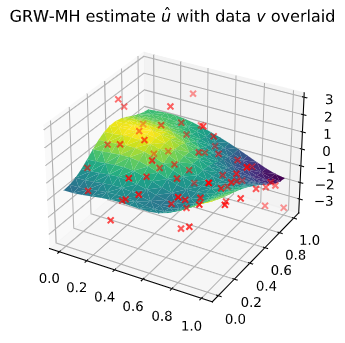
\includegraphics[width=\linewidth]{grw-mh-estimate.png}
		\caption{GRW-MH estimate}
		\label{fig:grw-estimate}
	\end{subfigure}
	\begin{subfigure}{0.31\linewidth}
		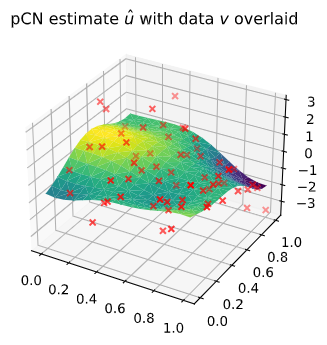
\includegraphics[width=\linewidth]{pcn-estimate.png}
		\caption{pCN estimate}
		\label{fig:pcn-estimate}
	\end{subfigure}
	\caption{Monte Carlo estimate errors ($D=16, T=10^4, \beta=0.2$)}
	\label{fig:u-estimate}
\end{figure}

The absolute error is plotted on figures \ref{fig:grw-err} and \ref{fig:pcn-err}. The error surface for each algorithm has a broadly similar shape (the mean absolute error is marginally higher for pCN). Indeed, by comparison with figure \ref{fig:v-2d}, the regions of high error are those in areas of sparse available data $\vbold$. This is to be expected as we cannot make a confident prediction in areas where we have few data-points.
%
\begin{figure}[!h]
	\centering
	\begin{subfigure}{0.32\linewidth}
		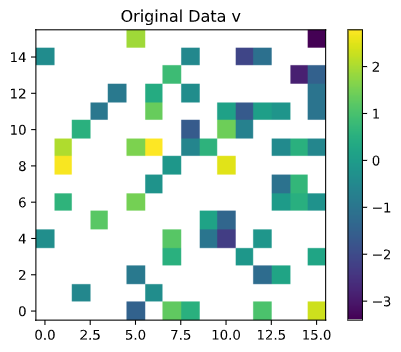
\includegraphics[width=\linewidth]{v-2d.png}
		\caption{Data $v$ projected onto X-Y plane}
		\label{fig:v-2d}
	\end{subfigure}
	\begin{subfigure}{0.32\linewidth}
		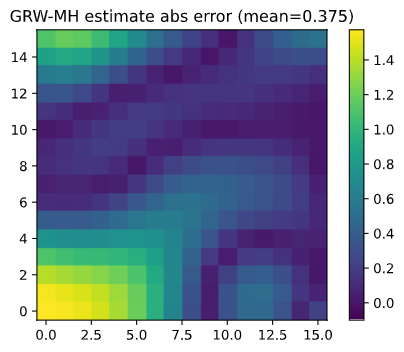
\includegraphics[width=\linewidth]{grw-mh-err.png}
		\caption{GRW-MH absolute error $|\hat{\ubold} - \ubold|$}
		\label{fig:grw-err}
	\end{subfigure}
	\begin{subfigure}{0.32\linewidth}
		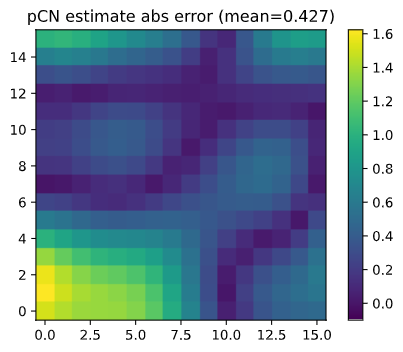
\includegraphics[width=\linewidth]{pcn-err.png}
		\caption{pCN absolute error $|\hat{\ubold} - \ubold|$}
		\label{fig:pcn-err}
	\end{subfigure}
	\caption{Monte Carlo estimate errors ($D=16, T=10^4, \beta=0.2$)}
	\label{fig:abs-error}
\end{figure}

The acceptance rate is an important measure of the wastefulness of the algorithm. We tabulate it in table \ref{tab:acceptance} for a range of grid-sizes $D$ and step-sizes $\beta$.
%
\begin{table}[!h]
	\centering
	\begin{tabular}{cc | cccc}
		Acceptance Rate    &    & \multicolumn{3}{c}{$\beta$}                    &  \\
		(GRW-MH $|$ pCN)       &    & 0.04          & 0.2           & 1.0            &           \\ \hline
		\multirow{2}{*}{D} & 4  & 0.932 $|$ 0.973 & 0.692 $|$ 0.886 & 0.054 $|$ 0.302 &           \\
		& 16 &   0.694 $|$ 0.851      &  0.097  $|$ 0.498         &    0.000 $|$  0.010  & 
	\end{tabular}
\caption{Acceptance rate for GRW-MH $|$ pCN algorithms for varying $\beta, D$}
\label{tab:acceptance}
\end{table}

Comparing the two algorithms, pCN has a higher acceptance for all tested scenarios. Higher dimensional spaces (larger $D$) necessarily have lower acceptance rates as there are more degrees of freedom so it is less likely that a random walk will move in a direction that increases the posterior (or likelihood for pCN). The acceptance rate for both algorithms decreases as $\beta$ increases. Nevertheless, having $\beta$ too low runs the risk of falling into a local optimum as there is insufficient energy to escape shallow wells. Therefore, it is less likely to converge to the true global optimum.

\subsection{Probit classification}

The model is now extended to work on a probit classification problem. The data $\vbold$ is put through a sign function to give the vector $\tbold$, such that $t_i \coloneqq \textrm{sign}(v_i) \in \{-1, +1\}$. As such the likelihood has the following form:
%
\begin{align}
	p(t_i = 1 | \ubold) &= p(v_i > 0 | \ubold) = p([G\ubold]_i + \epsilon_i > 0) \nonumber \\
	&= p(-\epsilon_i < \tilde{u}_i ) \nonumber \\
	&= \Phi(\tilde{u}_i)
\end{align}

Where $\Phi(\cdot)$ is the standard Gaussian CDF (as $-\epsilon_i \sim \epsilon_i \sim \Ncal(0,1)$). Note that the tilde denotes subsampling $\tilde{\ubold} \coloneqq G\ubold$. Conversely, for the case $t_i = -1$ the likelihood is given by:
%
\begin{align}
	p(t_i = -1 | \ubold) &= 1 - p(t_i = 1 | \ubold) \nonumber \\
	&= 1 - \Phi(\tilde{u}_i) \nonumber \\
	&= \Phi(-1 \cdot \tilde{u}_i)
\end{align}

This means we can simplify the expression for $t_i \in {-1, 1}$, leading to:
%
\begin{equation}
	p(t_i | \ubold_i) = \Phi(t_i \cdot \tilde{u}_i)
\end{equation}

We can extend this easily to find the likelihood $\lik(\cdot)$\footnote{Note that for simplicity we are not changing notation and all previous symbols in the $\vbold$ problem will retain their meaning for the $\tbold$ problem} of the latent variables $\ubold$ given the whole vector of observations $\tbold$:
%
\begin{align}
	\lik(\ubold) &= p(\tbold | \ubold) = \prod_{i=1}^{M} p(t_i | \ubold) = \prod_{i=1}^{M} \Phi(t_i \cdot \tilde{u}_i)
\end{align}

The second line arises from the fact that $t_i \indep t_j | \ubold$ or more specifically given $\tilde{\ubold} = G\ubold$. This a direct result of equation \ref{eqn:v-defn} as the noise terms $\epsilon_i$ are mutually independent. However, instead we find it easier to deal with the log-likelihood $\loglik(\cdot) \coloneqq \ln \lik(\cdot)$ as this turns the multiplication into a summation:
%
\begin{align}
	\loglik(\ubold) &= \sum_{i=1}^{M} \ln \Phi(t_i \cdot \tilde{u}_i) = \mathbf{1}^T \left[ \ln \Phi(\tbold \odot \tilde{\ubold}) \right]
	\label{eqn:log-lik-probit}
\end{align}

Where $\odot$ denotes element-wise multiplication of vectors, $\ln$ and $\Phi$ are extended to operate element-wise also and $\mathbf{1}$ is simply the vector of all-ones. This form in equation \ref{eqn:log-lik-probit} is very easy to implement using numpy as it is vectorised. With this log-likelihood function we can sample from the posterior $p(\ubold | \tbold)$ using pCN. From these samples we can perform a Monte Carlo estimate of the true class assignments for any $t^*_j$ not restricted to the subsampling imposed by $G$. The Monte-Carlo estimate is computed as follows:
%
\begin{align}
	p(t^*_j = 1 | \tbold) &= \int p(t^*_j = 1, \ubold | \tbold) d\ubold \nonumber \\
	&= \int p(t^*_j = 1 | \ubold) p(\ubold | \tbold) d\ubold \nonumber \\
	&\approx \frac{1}{T} \sum_{i=1}^{T} p \left( t^*_j = 1 | \ubold^{(i)} \right)
	\quad \textrm{for } \ubold^{(i)} \sim p(\ubold | \tbold) \nonumber \\
	&= \frac{1}{T} \sum_{i=1}^{T} \Phi \left( u^{(t)}_j \right)
\end{align}

It is important to note that both the $\tbold^*$ and $\ubold$ vectors are indexed by the same variable $j$, labelling position on the finite 2-D grid. We can quickly compute the vector of probabilities by dropping the $j$ dependence to give equation \ref{eqn:t-mc-estimate}.
%
\begin{equation}
	p(\tbold^* | \tbold) \approx \frac{1}{T} \sum_{i=1}^{T} \Phi \left( \ubold^{(i)} \right)
	\label{eqn:t-mc-estimate}
\end{equation}

This is a Monte-Carlo estimate, using the generated samples. We can plot the predictive probabilities on figure \ref{fig:t-predictive}. We see that the predictive distribution broadly follows the shape of figure \ref{fig:sign-u}. This is particularly impressive given the corruption apparent in figure \ref{fig:t-2d}.
%
\begin{figure}[!h]
	\centering
	\begin{subfigure}{0.32\linewidth}
		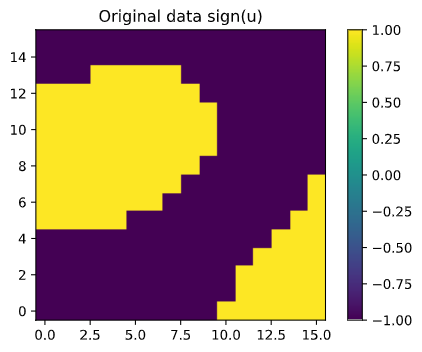
\includegraphics[width=\linewidth]{sign-u.png}
		\caption{True values $\tbold^* = \textrm{sign}(\ubold)$}
		\label{fig:sign-u}
	\end{subfigure}
	\begin{subfigure}{0.32\linewidth}
		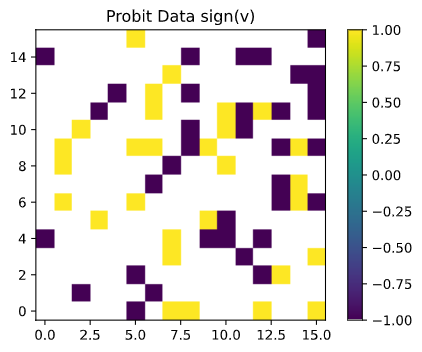
\includegraphics[width=\linewidth]{t-2d.png}
		\caption{Subsampled values after noise $\tbold$}
		\label{fig:t-2d}
	\end{subfigure}
	\begin{subfigure}{0.32\linewidth}
		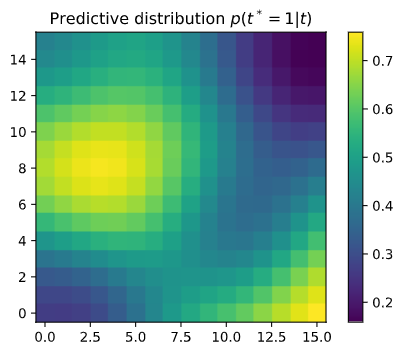
\includegraphics[width=\linewidth]{t-predictive.png}
		\caption{Predictive distribution $p(t^* = 1 | \tbold)$}
		\label{fig:t-predictive}
	\end{subfigure}
	\caption{Monte Carlo estimate of probit data ($D=16, T=10^4, \beta=0.2$)}
	\label{fig:t-estimate}
\end{figure}

\subsection{Length scale inference}

We now make hard assignments in the probit classification problem by thresholding at $p(t^*=1 | \tbold) = 0.5$ such that:
%
\begin{equation}
	\hat{t}^*_j = 
	\begin{cases}
		+1, & \text{if } p(t^*_j = 1 | \tbold) \geq 0.5\\
		-1,              & \text{otherwise}
	\end{cases}
\end{equation}
From this we can plot the absolute prediction error $|(\hat{t}^*_j - u_j)/2|$ and compute the mean $\eta$ over the index $j$ - which is equal to the probability of prediction error $\eta = p(t^*_j \neq \textrm{sign}(u_j))$ for general $j$. The hard assignments alongside the absolute errors are plotted in figure \ref{fig:t-hard-err}.
%
\begin{figure}[!h]
	\centering
	\begin{subfigure}{0.32\linewidth}
		
\includegraphics[width=\linewidth]{t-hard.png}
		\caption{Hard predictions $\hat{\tbold}^*$}
		\label{fig:t-hard}
	\end{subfigure}
	\begin{subfigure}{0.31\linewidth}
		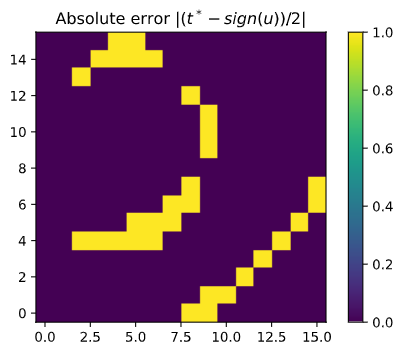
\includegraphics[width=\linewidth]{t-abs-error.png}
		\caption{Absolute error $|(\hat{t}^*_j - u_j)/2|$}
		\label{fig:t-err}
	\end{subfigure}
	\caption{Hard assignment prediction error ($D=16, T=10^4, \beta=0.2, l=0.3$)}
	\label{fig:t-hard-err}
\end{figure}

The plot in figure \ref{fig:t-err} gives a mean absolute error $\eta=0.125$. However, we wish to infer the length scale parameter $l$ by performing a line-search and minimising the mean absolute error $\eta$. This can be illustrated through a coarse logarithmic plot in the range $l \in [0.01, 10]$ and a finer linear plot in the range $l \in [0.2, 0.4]$ as in figures \ref{fig:l-coarse} and \ref{fig:l-fine} respectively.
%
\begin{figure}[!h]
	\centering
	\begin{subfigure}{0.32\linewidth}
		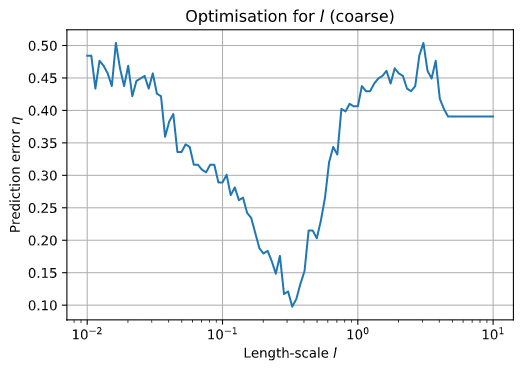
\includegraphics[width=\linewidth]{l-coarse.png}
		\caption{Coarse logarithmic scale}
		\label{fig:l-coarse}
	\end{subfigure}
	\begin{subfigure}{0.31\linewidth}
		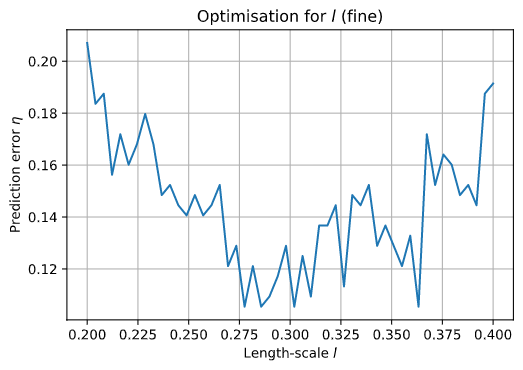
\includegraphics[width=\linewidth]{l-fine.png}
		\caption{Fine linear scale}
		\label{fig:l-fine}
	\end{subfigure}
	\caption{Prediction error $\eta$ against length-scale $l$}
	\label{fig:l-optimisation}
\end{figure}

It is rather computationally intensive to generate these plots in figure \ref{fig:l-optimisation}. We could instead perform a golden ratio line search to find the minimum. However, as each $\eta$ evaluation is non-deterministic the overall function would not be smooth for practical values of $n$ so this method is likely to have high error. By inspecting figure \ref{fig:l-fine} it is hard to obtain a point-estimate due to the uncertainty in each point. The best estimate would be $\hat{l} = 0.325 \pm 0.5$. This range encompasses the true value $l_0 = 0.3$. Therefore, inference in this case has succeeded.

Nevertheless, the method used to infer the estimate is hardly robust. A more generalisable approach can be obtained by returning to Bayes' rule in its full form and making explicit the dependence on length-scale $l$:
%
\begin{equation}
	p(\ubold | \tbold, l) = \frac{p(\ubold | l) \cdot p(\tbold | \ubold, l)}{p(\tbold | l)}
	\label{eqn:bayes}
\end{equation}

The term $p(\tbold | l)$ is independent of $\ubold$ and called the model evidence. It can be computed through a Monte-Carlo estimate as follows:
%
\begin{align}
	p(\tbold | l) &= \int p(\tbold | \ubold, l) \cdot p(\ubold | l) d\ubold = \int p(\tbold | \ubold) \cdot p(\ubold | l) d\ubold  \nonumber \\
	&\approx \frac{1}{T} \sum_{i=1}^{T} p(\tbold | \ubold^{(i)}) \quad \textrm{for } \ubold^{(i)} \sim p(\ubold | l) \nonumber \\
	&= \frac{1}{T} \sum_{i=1}^{T} \prod_{j=1}^{M} \Phi(t_j \cdot \tilde{u}^{(i)}]_j)
\end{align}

With this equation we can compute a Maximum-Likelihood estimate $\hat{l}^{ML} = \argmax_l p(\tbold | l)$; this is equivalent to maximising the model evidence. If we wanted to give $l$ a full Bayesian treatment, we would define a prior $p(l)$ and compute the posterior $p(l | \tbold) \propto p(l) \cdot p(\tbold | l)$. The posterior would be a complete probability distribution rather than a single point-estimate.

\section{Spatial Data}

We now turn our attention to real-world data. Specifically, we wish to develop a model to predict bike thefts in Lewisham borough based on spatial theft data. We have a series of 400m$^2$ cells identified by a $(x, y)$ coordinate and for each cell we have the total number of bike thefts within over 2015. This is denoted by a vector $\cbold$. For simplicity we use a tilde to denote the subsampled vectors $\tilde{\thetabold} \coloneqq G\thetabold$, $\tilde{\ubold} \coloneqq G\ubold$ and $\tilde{\cbold} \coloneqq G\cbold$. Once again, we emphasise that the original vectors have length $N$ which decreases to $M$ after the subsampling operation $G$.

\subsection{Poisson Likelihood}

We now deal with a Poisson likelihood. The field $\ubold$ is mapped to $\thetabold = \exp (\ubold)$ for positivity (there cannot be negative thefts in a region) and $\theta$ is used as the Poisson rate for each cell. The overall likelihood function is given below:
%
\begin{equation}
	p(\tilde{\cbold} | \thetabold) = \prod_{i=1}^{M} p(\tilde{c}_i | \tilde{\theta}_i)
	= \prod_{i=1}^{M} \frac{\exp (-\tilde{\theta}_i) \cdot \tilde{\theta}_i^{\tilde{c}_i}}{\tilde{c}_i!}
\end{equation}

As always we prefer to work with the log-likelihood giving us:
%
\begin{align}
	\ln p (\tilde{\cbold} | \thetabold) &= \sum_{i=1}^{M} \left( - \tilde{\theta_i} + \tilde{c}_i \ln \tilde{\theta}_i - \ln (\tilde{c}_i !) \right)
\end{align}

Substituting for $\thetabold = \exp (\ubold)$ we get:
%
\begin{align}
	\loglik(\ubold) &= \sum_{i=1}^{M} \left(- 
		\exp(\tilde{u}_i) + \tilde{c}_i \cdot \tilde{u}_i - \ln(\tilde{c}_i !)
	\right) \nonumber \\
	&= - \mathbf{1}^T \exp(\tilde{\ubold}) + \tilde{\cbold}^T \tilde{\ubold} - f(\tilde{\cbold})
	\label{eqn:log-lik-poisson}
\end{align}

We can ignore the term $f(\tilde{\cbold})$ for the purposes of pCN as it is independent of $\ubold$ and we are only interested in the difference of $\loglik$. Once we implement $\loglik(\ubold)$ we can use pCN to sample from the posterior $p(\ubold | \tilde{\cbold})$ with our standard operating parameters. Nevertheless, we must begin by guessing the length-scale parameter $l$ as this is not known in advance. This is covered in the subsequent section.

By way of reference, we plot the original bike theft field $\cbold$ and the subsampled data we feed to the pCN algorithm in figures \ref{fig:c-original} and \ref{fig:c-tilde} respectively.
%
\begin{figure}[!h]
	\centering
	\begin{subfigure}{0.32\linewidth}
		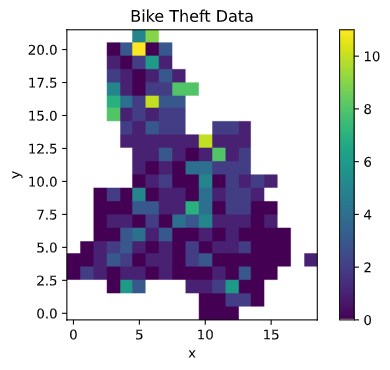
\includegraphics[width=\linewidth]{c-original.png}
		\caption{Original data $\cbold$}
		\label{fig:c-original}
	\end{subfigure}
	\begin{subfigure}{0.31\linewidth}
		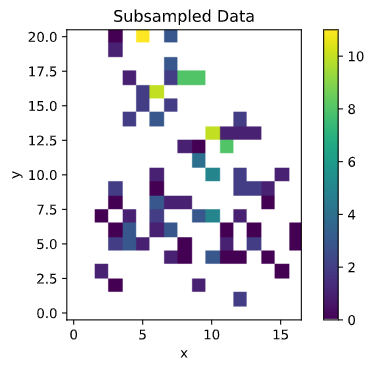
\includegraphics[width=\linewidth]{c-tilde.png}
		\caption{Subsampled data for pCN $\tilde{\cbold}$}
		\label{fig:c-tilde}
	\end{subfigure}
	\caption{Bike theft data for Lewisham}
	\label{fig:bike-theft-data}
\end{figure}

\subsection{Bike theft predictions}

We wish to estimate the expected counts $\hat{c}^*_j$ in each cell from the predictive distribution given the subsampled counts $\tilde{\cbold}$. The asterisk emphasises that this cell can have an arbitrary location not restricted to the subsampling imposed by $G$.
%
\begin{equation}
	\hat{c}^*_j \coloneqq \Expect \left[ c^*_j | \tilde{\cbold} \right] = \sum_{k=0}^{\infty} k \cdot p(c_j^* = k | \tilde{\cbold})
	\label{eqn:c-star-expect-start}
\end{equation}

The predictive distribution can be computed through a Monte-Carlo estimate as follows:
%
\begin{align}
	p(c_j^* = k | \cbold) &= \int p(c_j^* = k | \ubold) \cdot p(\ubold | \cbold) d\ubold \nonumber \\
	&\approx \frac{1}{T} \sum_{i=1}^{T} p(c_j^* = k | \ubold^{(i)}) \quad \textrm{for } \ubold^{(i)} \sim p(\ubold | \tilde{\cbold})
\end{align}

Substituting into equation \ref{eqn:c-star-expect-start} we can rearrange to obtain:
%
\begin{align}
	\hat{c}^*_j &\approx \sum_{k=0}^{\infty} k \cdot \frac{1}{T} \sum_{i=1}^{T} p(c_j^* = k | \ubold^{(i)}) \nonumber \\
	&= \frac{1}{T} \sum_{i=1}^{T} \sum_{k=0}^{\infty} k \cdot p(c^*_j = k | \theta^{(i)}_j) \nonumber \\
	&= \frac{1}{T} \sum_{i=1}^{T} \Expect \left[ c_j^* | \theta_j^{(i)} \right] \nonumber \\
	&= \frac{1}{T} \sum_{i=1}^{T} \theta_j^{(i)} \label{eqn:c-star-expect-final}
\end{align}

Where the last line holds as the expectation of a Poisson variable is simply its parameter. Therefore, we can perform pCN with the subsampled counts $\tilde{\cbold}$ to produce samples $\ubold^{(i)} \sim p(\ubold | \cbold)$. From these we can compute the expected count field by transforming $\thetabold^{(i)} = \exp (\ubold^{(i)})$ and applying equation \ref{eqn:c-star-expect-final}.

The first pass we perform uses the parameters $l=2, \beta=0.2, T=10^4$ and subsampling factor $f=3$. This yields the plots in figure \ref{fig:bike-predictions}. We see that these model settings yield an inferred field (figure \ref{fig:c-hat}) that roughly matches the empirical thefts in figure \ref{fig:c-original}. The hotspots are in the right locations but the choice of $l=2$ means that they leak into adjacent cells which does not happen frequently in the original dataset.
%
\begin{figure}[!h]
	\centering
	\begin{subfigure}{0.32\linewidth}
		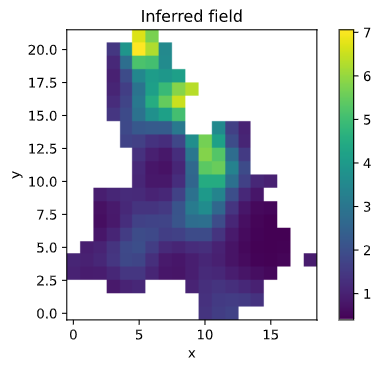
\includegraphics[width=\linewidth]{c-hat.png}
		\caption{Inferred field $\hat{\cbold}^*$}
		\label{fig:c-hat}
	\end{subfigure}
	\begin{subfigure}{0.32\linewidth}
		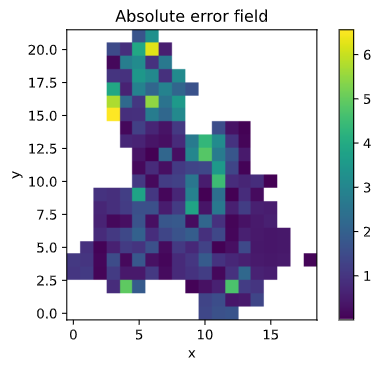
\includegraphics[width=\linewidth]{c-err.png}
		\caption{Absolute error field $|\hat{c}^*_j - c_j|$}
		\label{fig:c-error}
	\end{subfigure}
	\caption{Bike theft predictions ($l=2, \beta=0.2, T=10^4, f=3$)}
	\label{fig:bike-predictions}
\end{figure}

The absolute error field (figure \ref{fig:c-error}) has modest values but we see our predictions are thrown off in the Northern region. To be fair, this region sees large variations from cell-to-cell in the original data so we cannot expect a model with modestly large length-scale $l=2$ to predict all the cells well.

Lastly, we visualise the impact of extreme values of length-scale $l$ on the inferred field. This is plotted on figures \ref{fig:l-small} and \ref{fig:l-large}. The short length-scale (figure \ref{fig:l-small}) looks more similar to the true field in \ref{fig:c-original} however its greatest weakness is the subsampling. As the length-scale is so short $l=0.01$ adjacent cells (separated by a distance of 1) are basically independent. Therefore, this short length-scale struggles to fill in the gaps in the subsampled data. Indeed, all of the high count cells (above 5) appear in the subsampled dataset; the rest of cells draw little information from the subsampled dataset but are approximately distributed as the prior.
%
\begin{figure}[!h]
	\centering
	\begin{subfigure}{0.31\linewidth}
		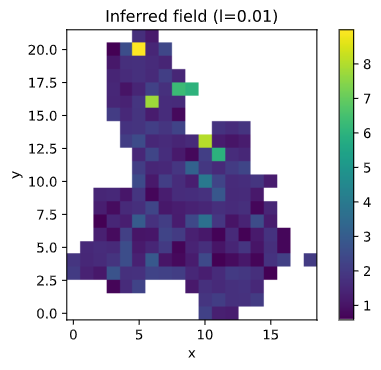
\includegraphics[width=\linewidth]{c-hat-l-small.png}
		\caption{Small length-scale $l=0.01$}
		\label{fig:l-small}
	\end{subfigure}
	\begin{subfigure}{0.32\linewidth}
		
\includegraphics[width=\linewidth]{c-hat-l-big.png}
		\caption{Large length-scale $l=100$}
		\label{fig:l-big}
	\end{subfigure}
	\begin{subfigure}{0.32\linewidth}
		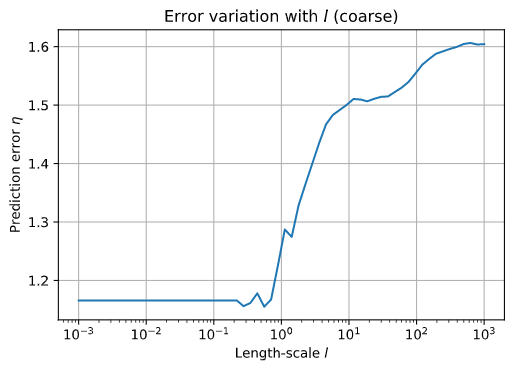
\includegraphics[width=\linewidth]{error-with-l.png}
		\caption{Absolute error field $|\hat{c}^*_j - c_j|$}
		\label{fig:error-with-l}
	\end{subfigure}
	\caption{Impact of length-scale $l$ on model performance}
	\label{fig:l-effect-bikes}
\end{figure}

The large length-scale $l=100$ on figure \ref{fig:l-big} only permits very slow variation. Indeed, all West-East variation is practically eliminated leaving only North-South variation. Clearly this does not fit the data well but could be a useful first order model.

We could choose $l$ by looking only at the mean absolute error (plotted in figure \ref{fig:error-with-l}) but this seems to favour very small values of length-scale as the observed data is rather noisy. Indeed, the choice of $l$ would best be suited by collecting further data for the model. Lewisham borough has an area of 35 km$^2$ meaning that each of the $N=207$ cells has side-length of approximately 400m. Now we would choose our length-scale $l$ to be the approximate radius in which a bike thief operates. This makes the suggestion of $l=2$ corresponding to 800m seem rather reasonable.

Indeed, we could apply a full Bayesian approach as in equation \ref{eqn:bayes} to inform our choice of $l$. This would necessarily involve a choice of prior informed by assumptions about bike thief radii of operation and an analysis of the model evidence $p(\tilde{c} | l)$.

\section{Conclusion}

In conclusion, we have shown that subsampling and inference using a Monte-Carlo Markoc-Chain (MCMC) can satisfactorily infer a latent field. Once the theory was shown to work on computer generated data we applied it to model bike thefts in Lewisham borough.

Indeed, the inferred field can be used to predict bike theft hotspots and removes much of the noise associated with real world data. This tool could be very useful for city planners or law enforcement officers seeking. However, the tools are very generic and can be applied to a whole host of other problems.
\end{document}
